
\marginpar{\href{https://youtu.be/CadZXGNauY0}{Video}}
\marginpar{\href{https://ocw.mit.edu/courses/6-041sc-probabilistic-systems-analysis-and-applied-probability-fall-2013/pages/unit-ii/lecture-9/}{Lecture Home}}
\marginpar{\href{https://ocw.mit.edu/courses/6-041sc-probabilistic-systems-analysis-and-applied-probability-fall-2013/0e64d4c45353c6ed659a2f5969407843_MIT6_041SCF13_L09.pdf}{Slides}}

Reading: 3.4-3.5

\marginpar{(6m)} Density is to be interpreted as probability per unit length at a certain place in the diagram

\marginpar{(7:20)}

Joint PDF $f_{X,Y}(x.y)$

\begin{align*}
P((X,Y) \in S) = \sum \sum_S f_{X,Y}(x.y)dx dy
\end{align*}

\begin{align*}
\int_{-\infty}^{\infty} \int_{-\infty}^{\infty} f_{X,Y} = 1, f_{X,Y} \ge 0
\end{align*}

From joint to marginal:
\begin{align*}
f_X(x) \cdot \delta \approx P(x \le X \le x + \delta) = \int_{-\infty}^{\infty} f_{X,Y}(x,y)dy
\end{align*}

\marginpar{(18:50)} Operational independence means you can multiply probabilities.

\subsection{Buffon's Needle}

\marginpar{(19m)}

\begin{figure}[h]
\centering
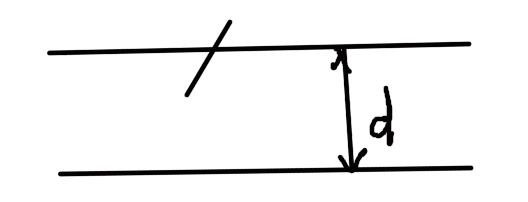
\includegraphics[width=5cm, height=4cm]{images/L09/buffon0.jpeg}
\caption{x}
\end{figure}

The needle can fall in one of two ways:

\begin{figure}[h]
\centering
\begin{minipage}{.45\linewidth}
  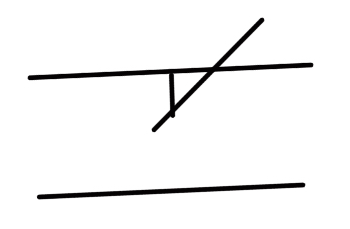
\includegraphics[width=\linewidth]{images/L09/buffon1.jpeg}
  \caption{Fall \#1}
  \label{bufffon1}
\end{minipage}
\hspace{.05\linewidth}
\begin{minipage}{.45\linewidth}
  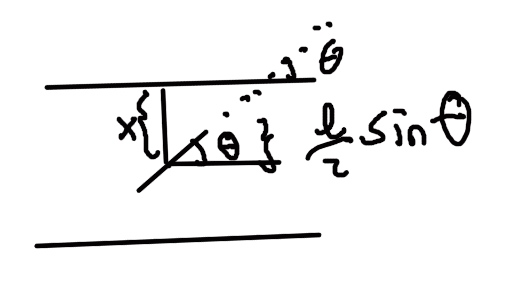
\includegraphics[width=\linewidth]{images/L09/buffon2.jpeg}
  \caption{Fall \#2}
  \label{bufffon2}
\end{minipage}
\end{figure}


\marginpar{(29m)}

Experimental measurement of Buffon's Needle problem.

\marginpar{(31m)}

Can interpret integral as a probability - simulation - Monte Carlo method

\subsection{Conditioning}

\marginpar{(31m)}

\subsection{Example: Stick-breaking}

\marginpar{(40:50m)}
